
%%%%%%%%%%%%%%%%% Intro %%%
\section{Introduction}
In this report various methods for the estimation of parameters of a given data set are evaluated and compared. To cut down the problem's complexity, we use a simple model for the flux of an elliptic galaxy, as is described by the Sersic profile, which provides us an initial data set. This data set - a noisy image of a elliptic galaxy as it would have been taken by a ground-based telescope - is then used to evaluate different estimation approaches as the least square estimation, maximum likelihood estimation and Bayesian estimation.\\
%Specifically, with these estimators the parameters for the flux of a galaxy is

\section{Modelling a galaxy}
The Sersic profile is very common amongst astrophysicists to model the flux of observed elliptic galaxies in a simple way, and is given by the equation

\begin{equation}
	\centering
	I(l,c) = exp(-R(l,c)^{\frac{1}{n}})
\end{equation}

which describes the variation of intensity with respect to the distance of the galaxy's centre.
The distance $R$ of a pixel with the coordinates $(l,c)$ from the galaxies centre is given by 

\begin{equation}
	\centering
	R(l,c)^2 = \bigg(\frac{(l-l_0)\sin(\alpha) - (c - c_0)\cos(\alpha)}{\sigma_l}\bigg)^2 + \bigg(\frac{(l-l_0)\cos(\alpha) - (c - c_0)\sin(\alpha)}{\sigma_c}\bigg)^2
\end{equation}

with $(l_0,c_0)$ being the galaxy's centre coordinates, $(\sigma_l,\sigma_c)$ the two galaxy's axes length and the horizontal angle $\alpha$.

This leads to the following equation modelling the data

\begin{equation}
	\centering
	d(l,c) = s + a I(l,c) + n(l,c)
\end{equation}

with $a$ as the amplitude of the galaxy, $s$ the amplitude of the sky's background and $n(l,c)$ as noise.

By assuming a white Gaussian noise with the known variance $\sigma_n^2$ and using the given Sersic-function (see Appendix \todo{add ref here}) we can create a "initial image" that will be used as the initial data set as previously mentioned, see figure \ref{img:initial}.
\begin{figure}[!h]
	\centering
	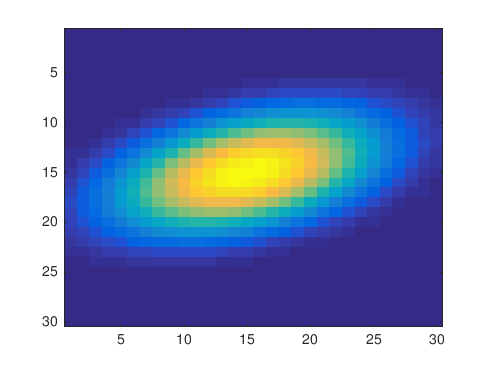
\includegraphics{images/galaxy_initial}s
	\label{img:initial}
	\caption{Initial Data Set, with a artificial elliptic galaxy}
\end{figure}

The parameters used to create fig. \ref{img:initial} are given below.

\begin{equation}
	\centering
	\begin{align*}
		L, C & = 30px & l_0, c_0 & = 15 & \sigma_l & = 10 & \sigma_c & = 5 \\
		\alpha & = 0.3 & n & = 0.4 & a & = 10 & s & = 3 
	\end{align*}
\end{equation}

with $L,C$ as height respectively width of image in pixels, $l_0, c_0$ the galaxy's centre in pixel coordinates and $\sigma_l, \sigma_c$ as length parameters.
\todo{probalby don't need this explananation here, see above text}


%%%%%%%%%%%%%%%%% TASK 1 %%%
\section{Estimation with known Galaxy's location and shape parameters}
Having successfully modelled a simple elliptic galaxy



%%%%%%%%%%%%%%%%% TASK 2 %%%
\section{Maximum likelihood estimation of all parameters}


%%%%%%%%%%%%%%%%% TASK 3 %%%
\section{Estimation in the Bayesian framework}

\subsection{Maximum a posteriori estimator}

\subsection{Posterior mean estimator}


